\chapter{Refactoring}
\label{ch:refactoring}
El refactoring del c\'odigo original se realiz\'o en Python 3.6 (versi\'on diferente a la que el programa fue implementado inicialmente: 2.7). Adem\'as se mantuvieron casi la totalidad de las librer\'ias cambiando \'unicamente Pymorph por Mahotas, debido a que la primera dej\'o de ser mantenida desde el 2010 y corresponde a la librer\'ia para Python 3.   

%\section{Ejecuci\'on de la rutina}
\section{Manejo de datos de entrada}
Toda las im\'agenes de entrada son manipuladas y servidas por la clase \textsc{DataPicker}. Esta clase se inicializa recibiendo un \textit{path} hacia un archivo de configuraci\'on (ver Ap\'endice \ref{subs:a1}) que contiene tanto las rutas a los archivos as\'i como los nombres de estos en t\'erminos de expresiones regulares, semestre a los que corresponde la secuencia de observaciones (los dos \'ultimos d\'igitos del a\~no concatenados con la letra A en caso de corresponder al primer semestre o B al segundo), el campo (representado como un n\'umero de dos d\'igitos, comenzando con cero para valores menores a 10) y el detector CCD (cadena de tres car\'acteres donde el primero de ellos describe a que grupo de detectores corresponde: N o S (ver figura \ref{fig:f4}); adem\'as de un n\'umero entero que va de 1 a 36) como strings. 
\bigskip

El archivo que esta clase consume, para la configuraci\'on de las rutas, debe contener los siguientes campos (ver ejemplo \ref{subs:a1}):
\begin{itemize}
\item \textbf{\texttt{maskDir}}: Directorio donde se almacenan las im\'agenes m\'ascara (im\'agenes que identifican p\'ixeles que no deben ser considerados).
\item \textbf{\texttt{scienceDir}}: Directorio donde se almacenan las im\'agenes cient\'ificas (im\'agenes base ya preprocesadas).
\item \textbf{\texttt{diffDir}}: Directorio donde se almacenan las im\'agenes de diferencia (resta entre las im\'agenes base y su cient\'ifica).
\item \textbf{\texttt{psfDir}}: Directorio donde se encuentran los modelos de psf (ap\'endice \ref{a1:psf}) usados para la determinaci\'on del flujo.
\item \textbf{\texttt{invDir}}: Directorio que guarda las im\'agenes correspondientes a la varianza inversa (\textit{peso} de cada pixel en t\'erminos de ruido: a menor peso, mayor ruido).
\item \textbf{\texttt{afluxDir}}: Directorio que contiene los archivos de extensi\'on \texttt{NPY} dentro de los cuales se guarda el valor de la variable \texttt{aflux}.
\item \textbf{\texttt{maskRegEx}}: Expresi\'on regular con la que es posible identificar el nombre de las im\'agenes m\'ascara en disco siguiendo el path \texttt{maskDir}.
\item \textbf{\texttt{scienceRegEx}}: Expresi\'on regular con la que es posible identificar el nombre de las im\'agenes cient\'ificas en disco siguiendo el path \texttt{scienceDir}.
\item \textbf{\texttt{diffRegEx}}: Expresi\'on regular con la que se identifican el nombre de las im\'agenes de diferencia en disco siguiendo el path \texttt{diffDir}.
\item \textbf{\texttt{invRegEx}}: Expresi\'on regular con la que es posible identificar el nombre de las im\'agenes de la varianza inversa siguiendo el path \texttt{invDir}.
\item \textbf{\texttt{afluxRegEx}}: Expresi\'on regular con la que se identifica el nombre de los archivos \textit{match} que contienen el valor de \texttt{aflux}. Estos archivos est\'an ubicados en el path \texttt{afluxDir}.
\item \textbf{\texttt{psfRegEx}}: Expresi\'on regular que describe el nombre de las im\'agenes que guardan el modelo de PSF en el directorio \texttt{psfDir}.
\end{itemize}


\textsc{DataPicker} maneja  la lectura y preparaci\'on de las im\'agenes a ser analizadas, mientras que un segundo proceso correspondiente a la lectura de resultados anteriores (guardados en un archivo de texto plano) se describir\'a en el Cap\'itulo 5 de nuevas funcionalidades \ref{ch:news}. 
\bigskip
  
\subsection{Lectura y preparaci\'on de im\'agenes}
A continuaci\'on se enumeran los diferentes m\'etodos que intervienen en la recolecci\'on de los datos a ser le\'idos:

\begin{itemize}
\item \textbf{\texttt{config\_reg\_expressions(semester, field, ccd)}}\\
Este m\'etodo recibe como par\'ametros strings que indiquen el semestre (\texttt{semester}), el campo (\texttt{field}) y el ccd (\texttt{ccd}) que se quiere analizar. Puede hacerse uso de los valores de las variables de instancia que la misma clase \textsc{DataPicker} recibe en su constructor. Con estos strings se establecen las rutas de los directorios de las im\'agenes y las expresiones regulares de los nombres de las mismas.
\bigskip

\item \textbf{\texttt{collect\_data()}}\\
Esta funci\'on se encarga de recolectar la ruta completa de las diferentes im\'agenes (m\'ascaras, im\'agenes cient\'ificas, de diferencia, etc.). Para esta finalidad se hace uso del m\'etodo \texttt{walking\_through\_files}. 
\bigskip

\item \textbf{\texttt{walking\_through\_files(regex, dir)}}\\
M\'etodo con el cual se recorren las rutas definidas en los pasos anteriores y se agrupan los nombres completos (directorio incluido) de las im\'agenes ubicadas en el directorio \texttt{dir} y posean un nombre de patr\'on que siga la expresi\'on regular \texttt{regex}.
\bigskip

\item \textbf{\texttt{filter\_science\_images()}}\\
Filtra im\'agenes cient\'ificas de acuerdo a su airmass (Ap\'endice  \ref{ap:airmass}), seleccionando aquellas obtenidas en fechas cuyo valor de airmass calculado es menor a 1,7. De esta secuencia de im\'agenes cient\'ificas resultante se obtiene una lista de fechas que cumplen esta condici\'on medidas en t\'erminos de \textit{d\'ia juliano modificado} o \textit{Modified Julian Date} (MJD) de tipo punto flotante. Estos valores son ordenados de forma creciente.%las fechas en que las observaciones fueron hechas en t\'erminos de \textit{d\'ia juliano modificado} o \textit{Modified Julian Date} (MJD) como variables de punto flotante.
\bigskip

\item \textbf{\texttt{select\_fits(dir)}}\\
Selecciona y ordena los elementos de la lista de im\'agenes de formato fits del directorio \texttt{dir} usando la lista de MJDs (guardada en la variable de instancia \texttt{mjd} de la clase) generada en \texttt{filter\_science\_images()} escogiendo s\'olo aquellas cuyas fechas correspondan a las fechas indicadas.  %cronol\'ogico (i.e. de acuerdo a la secuencia de MJD encontrada en \texttt{filter\_science\_images()}).
\bigskip

\item \textbf{\texttt{select\_npys(dir, ref\_dir, init\_index, n\_pos, rest\_len)}}:\\
Debido a que los archivos de extensi\'on NPY no poseen la variable MJD en su estructura (en los archivos FITS encontramos este valor en el header de la imagen) deben de filtrarse de forma diferente. Para este caso el filtrado de este tipo de archivos se lleva a cabo a trav\'es de la revisi\'on de sus nombres, ya que comparten patrones con los nombres de ciertas im\'agenes fits. Por ejemplo, los nombres de las im\'agenes de PSF, de formato NPY, poseen similitud con los nombres de las im\'agenes FITS de diferencia; igualmente los archivos \texttt{aflux} de formato NPY poseen parecidos en sus nombres con las im\'agenes cient\'ificas. Este parecido es medido a trav\'es de un substring diferente para cada tipo de archivo NPY, definido por la posici\'on inicial \texttt{init\_index}, en el nombre del archivo FITS y largo \texttt{rest\_len}. \texttt{n\_pos} indica la posici\'on de un car\'acter espec\'ifico `` \_ '' en dicho substring para validar esta comparaci\'on.
%Selecciona los archivos de extensi\'on NPY que se encuentran en el directorio \texttt{dir}. Los nombres son filtrados en relaci\'on a las im\'agenes listadas de \texttt{ref\_dir} seg\'un el paso de \texttt{select\_fits(dir)} (es decir, debe ser un directorio que contenga im\'agenes FITS). \texttt{init\_index}, \texttt{n\_pos} y \texttt{rest\_len} son enteros usados para extraer substrings espec\'ificos de los nombres de los archivos.
\end{itemize}

\section{Determinaci\'on de flujos}
El c\'alculo del flujo, en este refactoring, se independiz\'o del manejo de archivos (en el programa orginal estaba alojado en la clase \textsc{FITSHandler}) y se implement\'o en el script \texttt{utils} pensado como librer\'ia.
%El proceso de la obtenci\'on del flujo se simplific\'o, eliminando la clase FitsHandler del programa original. Debido a la posibilidad de hacer los m\'etodos de esta clase est\'aticos se implement\'o un script Python denominada \texttt{utils} para contener estas rutinas e implementarlas est\'aticamente.
\bigskip

Los m\'etodos que participan en la rutina de calculo de flujo son: 

\begin{itemize}
\item \textbf{\texttt{naylor\_photometry(invvar, diff, psf)}\cite{naylor}:}\\
Calcula el producto del flujo por su varianza. Retorna el producto y la varianza. Para esto obtiene el flujo a partir de la imagen PSF entregada (\texttt{psf}) y del producto entre la imagen diferencia y la de varianza inverza (\texttt{diff} y \texttt{invvar} respectivamente).
\bigskip


\item \textbf{\texttt{calc\_fluxes(diff, psf, invvar, aflux)}:}\\
Calcula el flujo y su varianza gestionando la entrada y la salida de \texttt{naylor\_photometry(invvar, diff, psf)}. Los valores NaN son transformados a valores de punto flotante de constante 0.001.
\end{itemize} 

Estos m\'etodos  son llamados desde la rutina \textsc{RoutineHandler} (ver Cap\'itulo \ref{ch:news}).
\section{Filtros originales}
La refactorizaci\'on de los filtros de Kalman originales implic\'o la implementaci\'on de nuevas clases e interfaces para el desarrollo del patr\'on propuesto: Strategy (ver familia de m\'etodos resultante en la figura \ref{fig:ref1}). A continuaci\'on se presentan cada una de ellas:

\begin{itemize}
\item \textbf{IPredict:} Interface que describe el comportamiento de la funci\'on \textsc{Predict} de un filtro de Kalman. \texttt{predict} recibe como par\'ametros el paso de tiempo ($\Delta t$), la matriz de estado, la matriz de covarianza de estado, y las predicciones de las matrices de estado y covarianza determinadas en el paso anterior (con la finalidad de actualizar estas variables). Su firma queda como:
\begin{center}
\texttt{predict(delta\_t, state, state\_cov, pred\_state, pred\_cov)}
\end{center}
Este m\'etodo entrega finalmente las matrices de estado y covarianza de estado predicho.
\bigskip

\item \textbf{ICorrect:} Interface que describe el comportamiento de la funci\'on \textsc{Correct} de un filtro de Kalman. \texttt{correct} recibe como par\'ametros el matriz de flujo (\texttt{z}) y de varianza de las observaciones (\texttt{R}), la matriz de estado predicha, la matriz de covarianza predicha, la matriz de estado y la matriz de covarianza (para sobreescritura) obtenidas en el paso anterior. Su firma queda como:
\begin{center}
\texttt{correct(z, R, pred\_state, pred\_cov, state, state\_cov)}
\end{center}
\bigskip
Esta funci\'on entrega finalmente las matrices de estado y covarianza de estado corregido.

\end{itemize}

\subsection{Predicci\'on}
\textbf{LinearPredict:} Clase que extiende de IPredict. Implementa m\'etodo \texttt{predict} que ser\'a usado tanto por el filtro b\'asico como el de m\'axima correntrop\'ia. Su instanciaci\'on recibe como argumento \texttt{sigma\_a} (desviaci\'on est\'andar del modelo, asumiendo una distribui\'on gaussiana en la distribuci\'on de las observaciones).
\bigskip


\subsection{Correcci\'on}
\textbf{BasicCorrect:} Clase que extiende de ICorrect. Implementa m\'etodo \texttt{correct} que ser\'a usado para el tipo de filtro de Kalman B\'asico.
\bigskip

\textbf{MCCorrect:} Clase que extiende de ICorrect. Implementa m\'etodo \texttt{correct} que ser\'a usado para el tipo de filtro de Kalman de m\'axima correntrop\'ia. El constructor de esta clase recibe los siguientes par\'ametros:

\begin{itemize}
\item \texttt{epsilon}: Cantidad con la cual se contrastar\'a el error o precisi\'on que se quiera lograr con la estimaci\'on.
\item \texttt{max\_iter}: N\'umero m\'aximo de iteraciones.
\item \texttt{silverman}: \textit{boolean}. Determina si se usa o no la apoximaci\'on de Silverman para el ancho de banda del kernel Gaussiano.
\item \texttt{std\_factor}: Factor de desviaci\'on est\'andar usado en la aproximaci\'on de Silverman.
\item \texttt{sigma}: Sigma usado para el kernel Mercer.
\end{itemize}

\subsection{Filtros refactorizados}

\begin{itemize}
\item \textbf{KalmanFilter:} Clase abstracta padre de los subtipos BasicKalmanFilter y MCKalmanFilter. Posee los m\'etodos abstractos \texttt{predict} y \texttt{correct}, que son definidos de acuerdo a las estrategias de predicci\'on y correci\'on descritas previamente.
\item \textbf{BasicKalmanFilter:} Representa el filtro b\'asico de Kalman. Est\'a compuesto por las estrategias \texttt{LinearPredict} y \texttt{BasicCorrect}.
\item \textbf{MCKalmanFilter:} Representa el filtro de m\'axima correntrop\'ia. Est\'a compuesto por las estrategias \texttt{LinearPredict} y \texttt{MCCorrect}.
\end{itemize}
\bigskip

\begin{figure}
\centering
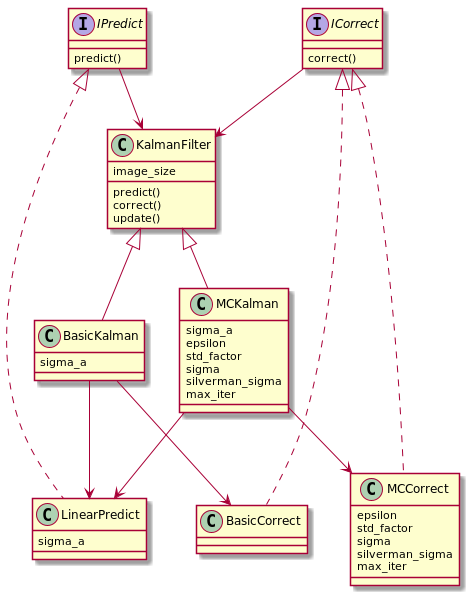
\includegraphics[scale=.5]{images/kalmanfilter_class}
\caption{Familia de filtros de Kalman y patr\'on \textit{strategy} usado en la implementaci\'on de los m\'etodos \texttt{predict} y \texttt{correct}.}
\label{fig:ref1}
\end{figure}

\section{Detecci\'on de candidatos}
Mientras que la detecci\'on de candidatos en el programa original se realiza en una instancia de la clase \textsc{SNDetector}, la detecci\'on en la nueva versi\'on se realiza en SourceFinder, el cual funciona de la misma forma que su antecesor. El cambio de nombre representa la intencionalidad de extender la funcionalidad de esta clase no s\'olo a la detecci\'on de supernovas sino adem\'as encontrar objetos como estrellas variables.
\bigskip

Su constructor requiere los siguientes argumentos:
\begin{itemize}
\item \texttt{flux\_thresh:} Umbral de corte para el flujo estimado por el filtro de Kalman.
\item \texttt{flux\_rate\_thresh:} Umbral de corte de velocidad de flujo estimado por el filtro de Kalman.
\item \texttt{rate\_satu:} Tasa de saturaci\'on en la velocidad de flujo.
\item \texttt{accum\_neg\_flux\_depth:} Cantidad de \'epocas de registro de p\'ixeles negativos (para la construcci\'on de una matriz de booleans de esta profundidad).
\item \texttt{accum\_med\_flux\_depth:}: Cantidad de \'epocas de registro de p\'ixeles cuya intensidad mediana (durante las \'epocas) es mayor a 1500.
\item \texttt{image\_size:} Dimensi\'on de las im\'agenes FITS.
\item \texttt{n\_consecutive\_obs:} N\'umero de alertas u observaciones consecutivas a considerar para confirmar una detecci\'on.

\end{itemize}
%La detecci\'on de candidatos en el programa original se realiza en \textsc{SNDetector}, sin embargo, durante este refactoring se descompuso el proceso de reconocimiento de fuentes estelares (grupo de pixeles brillantes) del proceso de selecci\'on de candidatos, siendo este \'ultimo la continuaci\'on del primero. Por tanto se crearon las clases \textsc{SourceFinder} para el filtrado y agrupamiento de pixeles y \textsc{TPDetector} (transient phenomena detector) para la revisi\'on de las \textit{fuentes} encontradas en el paso anterior.
\subsection{SourceFinder}
La clase \textsc{SourceFinder} posee los siguientes m\'etodos:
\begin{itemize}
\item \texttt{pixel\_discard}:\\
M\'etodo en el que se realiza el descarte de p\'ixeles de forma individual, siguiendo los siguientes criterios:
\begin{enumerate}
\item Si el flujo estimado por el filtro de Kalman para un pixel es menor que el umbral dado.
\item Si la velocidad de flujo estimada por el filtro de Kalman es menor que el umbral  de la velocidad de flujo multiplicado por un factor determinado la tasa de saturaci\'on en la velocidad de flujo y el flujo estimado por el filtro.
\item Si un pixel de la imagen cient\'ifica es menor a la mediana m\'as cierto delta (en este trabajo, siguiendo la l\'inea de desarrollo de P. Huentelemu \cite{huentelemu}, se consider\'o 5.0) es descartado.
\item Si las varianzas de flujo son mayores a 150.0 (valor estimado por el autor del software original \cite{huentelemu}).
\item Si las varianzas de la tasa de cambio de flujo (o velocidad de flujo) es mayor o igual a 150.0.
\item Si los p\'ixeles no caen en etiquetas de invalidaci\'on dentro de la m\'ascara que ha sido procesada para marcar tambi\'en los p\'ixeles vecinos a los realmente defectuosos.
\item Si los p\'ixeles no han ca\'ido dentro del descarte por superar la mediana estimada a partir de cuatro \'epocas. 
\end{enumerate}
\item \texttt{grouping\_pixels()}:\\
Este m\'etodo trabaja con las etiquetas determinadas en el paso anterior en un arreglo de matrices (\texttt{numpy array}) denominado \texttt{pixel\_flags} (variable de instancia). Adem\'as recibe el \'indice de MJD correspondiente a la observaci\'on de tal fecha.
La agrupaci\'on de p\'ixeles se realiza gracias a funciones brindadas por la librer\'ia \textsf{Mahotas}, usando el m\'etodo \texttt{label} para encontrar dominios cerrados en el mapa de p\'ixeles validados.
\bigskip

\item \texttt{filter\_groups(science, flux, var\_flux, state, base\_mask)}:\\
Este m\'etodo recibe la imagen cient\'ifica, el flujo y su varianza, el estado determinado por el filtro de Kalman y la m\'ascara correspondiente a una \'epoca espec\'ifica. 
El filtrado de grupos de p\'ixeles se lleva a cabo bajo las siguientes reglas de descarte: 

\begin{enumerate}
\item Descarte de grupo por contener posible mala resta alrededor (valores negativos).  
\item	Si no hay m\'aximos locales dentro del grupo de p\'ixeles encontrados dentro de la imagen cient\'ifica.
\item	Si no hay m\'aximos locales dentro del grupo de p\'ixeles encontrados dentro de la matriz de flujo (calculado por \texttt{calc\_fluxes}).
\item	Si no hay m\'aximos locales dentro del grupo de p\'ixeles encontrados dentro de la matriz velocidad de flujo.
\item 	Si los valores de los p\'ixeles superan la mediana local en imagen cient\'ifica.
\item	Si el grupo posee alg\'un pixel que doble el valor del flujo o de la imagen cient\'ifica.
\item	Si el centro del grupo se encuentra etiquetado como defectuoso dentro de la m\'ascara.
\item	Si el pixel del centro del grupo se encuentra rechazado al ser superior a la mediana de los p\'ixeles de cuatro observaciones consecutivas.
\item	Si la varianza del flujo del pixel del centro del grupo es mayor al determinado por el umbral.
\end{enumerate} 
\item \texttt{update\_candidates(mjd):}\\
En la estructura \texttt{CandData} se van registrando fechas (MJD) en que se han detectado candidatos previamente o se han detectado por primera vez. Es una estrutura tipo lista en la que se van guardando diccionarios que contienen, cada uno, las coordenadas de un objeto, las \'epocas en las que ha sido detectado y si corresponde o no a una supernova conocida.

\item \texttt{check\_candidates(SN\_index, SN\_pos):}\\
Verifica que dado un \'indice de supernova (\texttt{SN\_index}) y sus coordenadas \texttt{SN\_pos} se ha detectado dentro de los candidatos encontrados. 

\item \texttt{draw\_complying\_pixel\_groups(science, state, state\_cov, base\_mask, dil\_mask, flux, var\_flux, mjd)}:\\
Este m\'etodo es el que llama a \texttt{pixel\_discard} para etiquetar p\'ixeles para el descarte y no ser considerados en el paso de agrupamiento al llamar a \texttt{grouping\_pixels}. Luego se invoca el m\'etodo \texttt{filter\_groups} para hacer el descarte a nivel grupal y obtener candidatos. La \'ultima llamada es para el m\'etodo \texttt{update\_candidates} para actualizar lista de candidatos encontrados en la variable de instancia \texttt{CandData}.
\bigskip

Como argumentos recibe todos los elementos necesarios para ejecutar los m\'etodos que llama.
%\texttt{save\_data} que se encuentra en clase \textsc{DataContent}. 

\end{itemize}

\section{Visualizaci\'on de resultados}
En el proceso de visualizaci\'on participan dos clases: \textsc{Observer} y \textsc{Visualizer}. La primera clase es la encargada de generar una lista de diccionarios dentro de los cuales se almacena informaci\'on de los candidatos encontrados durante el proceso de detecci\'on. Esta lista es guardada como una variable de instancia en \textsc{Observer} denominada \texttt{objects} y la informaci\'on contenida por cada uno de los diccionarios corresponde a las siguientes componentes:

\begin{itemize}
\item Ubicaci\'on del objeto en la primera imagen cient\'ifica procesada, como un arreglo de \textit{floats} de largo dos. 
\item Lista de \'epocas en las que el objeto fue detectado.
\item Listas de estampillas de diferente profundidad, de ancho y alto $21 \times 21$. Las estampillas de cada lista tendr\'an una profundidad propia dependiendo de la estructura que est\'en almacenando. Estas estructuras pueden ser im\'agenes como la cient\'ifica, de diferencia, m\'ascara, etc., o a estructuras como las etiquetas de p\'ixeles grupales e individuales, matrices de estado, etc. Cada una de las estampillas de cada lista corresponder\'a a la medici\'on, c\'alculo o estimaci\'on obtenida para una \'epoca espec\'ifica. Adem\'as cada una de las estampillas est\'a centrada en la coordenada del objeto candidato a revisar.   
\end{itemize}
%En la visualizaci\'on de la informaci\'on de los candidatos participan dos clases: \textsc{Observer} y \textsc{Visualizer}. Con una instancia de la primera clase, se generan listas de \textit{estampillas} $21\times21$ (matrices) centradas en las coordenadas de los candidatos para las diferentes estructuras como imagen cient\'ifica, flujo, estimaci\'on de flujo obtenida por el filtro de Kalman, etc. Estos datos son guardados en una lista de diccionarios: \texttt{obj}. En los diccionarios est\'an contenidos estas series de estampillas, adem\'as de la posici\'on y \'epocas de detecci\'on de un candidato espec\'ifico.
\bigskip

Para el registro de estos datos se emplean dos m\'etodos de \textsc{Observer} listados a continuaci\'on:

\begin{itemize}
\item \texttt{set\_space (cand\_data):}\\
Recibe lista de candidatos (coordenadas) \texttt{cand\_data} y crea lista de diccionarios, \texttt{objects}, para guardar la informaci\'on de los primeros para todas las \'epocas analizadas creando arreglos (de la librer\'ia \textsc{Numpy}) de estampillas $21 \times 21$ destinadas a guardar los datos de las diferentes estructuras: im\'agenes, matrices de estado estimado y predicho, covarianzas por pixel, matrices de etiquetas de p\'ixeles, etc. Cada estampilla estar\'a centrada en la posici\'on del candidato en la primera imagen cient\'ifica analizada. 
\bigskip

\item \texttt{look\_candData(cand\_data, pred\_state, pred\_state\_cov, kalman\_gain, state, state\_cov, time\_mjd, flux, var\_flux, science, diff, psf, base\_mask, dil\_base\_mask, pixel\_flags, pixel\_group\_flags, mjd\_idx):}\\

Con el espacio generado en la estructura \texttt{objects}, se procede a ejecutar la pipeline principal (calculo de flujo, generaci\'on de estimaciones con filtro de Kalman y proceso de detecci\'on) para, en esta ocasi\'on, ir guardando resultados de los candidatos en \texttt{cand\_data} en su diccionario respectivo por cada \'epoca (cuyo \'indice est\'a representado por el argumento \texttt{mjd\_idx}). Por tanto recibe como argumentos las matrices de estados y covarianzas predichos (\texttt{pred\_state} y \texttt{pred\_state\_cov} respectivamente), las matrices de estados y covarianzas estimados (\texttt{state} y \texttt{state\_cov}) la matriz de ganancia de Kalman (\texttt{kalman\_gain}), matriz de flujo calculado y varianza asociada (\texttt{flux} y \texttt{var\_flux}), imagen cient\'ifica (\texttt{science}) y de diferencia (\texttt{diff}), imagen de la PSF usada (\texttt{psf}), matrices de etiquetas de p\'ixeles (\texttt{pixel\_flags} y \texttt{pixel\_group\_flags}) e imagen de la m\'ascara usada (base\_mask) junto a su versi\'on post-proceso de dilataci\'on (dil\_base\_mask).


\item \texttt{plot\_results(semester, field, ccd, plots\_path)}\\
Finalmente, con la variable de instancia \texttt{objects} lista, es posible generar los gr\'aficos de cada candidato con este m\'etodo, el cual recibe como par\'ametros el semestre (\texttt{semester}), el campo (\texttt{field}) y el CCD (\texttt{ccd}) de donde se obtuvieron las im\'agenes junto a la ruta al directorio donde se quiere guardar las im\'agenes (\texttt{plots\_path}) como argumentos. Los gr\'aficos son generados por una instancia de la clase \textsc{Visualizer}.
 %La clase \texttt{Visualizer} es la encargada de generar las im\'agenes de los gr\'aficos. 
\end{itemize}

 
La clase \textsc{Visualizer} permite la obtenci\'on de tres tipos gr\'aficas de acuerdo al m\'etodo llamado.
 
\begin{itemize}
  
\item \textbf{Estampillas}\\ 
Se muestra el comportamiento de los p\'ixeles en las estampillas de dimensi\'on $21 \times 21$ de las siguientes estructuras: imagen cient\'ifica, PSF, flujos observado y su varianza, estados de flujo y su velocidad estimados por filtro de Kalman, etiquetas grupales e individuales de p\'ixeles.
\item \textbf{Curva de estado}\\
 Esta curva se logra a partir de los valores estimados de flujo y de las velocidad de esta obtenidos por el filtro de Kalman. Esta gr\'afica muestra la complejidad de la curva visualizada calculando su entrop\'ia \cite{balestrino}.
\end{itemize}

Estas gr\'aficas son generadas gracias a los siguientes m\'etodos de \textsc{Visualizer}:

\begin{itemize}
\item \texttt{print\_lightcurve(obj, obs\_rad, figsize1, figsize2, save\_filename):}\\

Este m\'etodo est\'a destinado a crear series de tiempo, para contrastar, de diferentes variables de inter\'es tales como el flujo observado, estimado y predicho (medidos en el pixel central del candidato) visualizadados en la misma gr\'afica. Del mismo modo, en un gr\'afico dispuesto bajo el primero, se dibuja las series de tiempo de las velocidades estimadas y predichas. Posteriormente se grafica la evoluci\'on de las etiquetas de p\'ixeles individuales y grupales, y el \'ultimo gr\'afico generado corresponde a la serie de tiempo de las varianzas y covarianzas de las diferentes variables como flujo, estimaciones de flujo y sus predicciones obtenidas con el filtro de Kalman, etc.
\bigskip

 Los par\'ametros \texttt{figsize1} y \texttt{figsize2} corresponden a la altura y ancho de la imagen generada. Por \'ultimo, \texttt{save\_filename} corresponde al nombre con el que se guardar\'a el archivo en disco en formato PNG. Ejemplo de imagen resultante en figura \ref{fig:lc_result}.
%\bigskip
 
\item \texttt{print\_stamps(obj, figsize1, figsize2, save\_filename):}\\
Recibe como entrada un diccionario de la lista de objetos almacenados por una instancia de \textsc{Observer}. Con esta funci\'on las estampillas son impresas secuencialmente (orden cronol\'ogico) en filas, donde cada una de estas \'ultimas corresponde a alg\'un tipo de imagen o estructura como la imagen cient\'ifica, estimaci\'on de flujo, etiquetas de p\'ixeles, etc. (ver ejemplo de imagen en figura \ref{fig:stamps_result}).
\bigskip

Los valores \texttt{figsize1} y \texttt{figsize2} corresponden a la dimensi\'on de la imagen resultante. El argumento \texttt{save\_filename} indica el nombre con el que se quiere guardar el documento (de formato PNG) en disco. 
%Recibe el nombre del archivo con el cual se guardar\'a la imagen. Es la funci\'on encargada de construir la imagen donde se muestra la evoluci\'on de los flujos y las etiquetas de los pixeles en diferentes etapas en las estampillas obtenidas previamente .
\item \texttt{print\_space\_states(obj, obs\_rad, figsize1, figsize2, flux\_thresh, rate\_flux\_thresh, save\_filename):}\\
Esta funci\'on es la encargada de graficar la curva de estados por los que pasa un candidato (cuya informaci\'on est\'a contenida en el diccionario \texttt{obj}). Se visualizan los estados de  tres \'epocas anteriores junto a los estados de las \'epocas en que ocurre su detecci\'on (mientras dure la alerta de detecci\'on). Estos estados est\'an definidos por pares de valores de flujo y velocidad de flujo estimado por el filtro de Kalman. Adem\'as en la misma imagen, se indica el nivel de complejidad de la curva en t\'erminos de entrop\'ia \cite{balestrino}. Un ejemplo de imagen resultante se observa en la figura \ref{fig:sp_st}.
\bigskip

Los argumentos del m\'etodo, \texttt{figsize1} y \texttt{figsize2}, corresponden a las dimensiones de alto y ancho de la imagen a generar, mientras que \texttt{save\_filename} indica el nombre del archivo generado a guardar.  
\end{itemize}

\begin{figure}[h!]
\centering
\includegraphics[scale=.45]{/home/paloma/Documents/PLOTS/BASIC/lc_sem_15A_field_38_ccd_S25_obj_1.png}
\caption{Conjunto de series de tiempo de diferentes componentes de inter\'es en el pixel ubicado en la coordenada de posici\'on del candidato. El primer gr\'afico (de arriba hacia abajo) muestra la evoluci\'on del flujo medido en contraste con el comportamiento del la predicci\'on y estimaci\'on realizada por el filtro de Kalman del mismo flujo durante las \'epocas de las observaciones . La segunda visualizaci\'on muestra los cambios de la predicci\'on y estimaci\'on de la velocidad de flujo (obtenidas por el filtro de Kalman) en el tiempo. El tercer esquema muestra la evoluci\'on de las etiquetas (grupal e individual) del pixel ubicado en la coordenada del candidato. Finalmente, el \'ultimo gr\'afico visualiza el comportamiento de las diferentes varianzas y covarianzas tanto de las componentes predichas y estimadas por el filtro (flujo y velocidad de flujo) as\'i como de las mediciones del mismo flujo (observado).}
\label{fig:lc_result}
\end{figure}

\begin{figure}[h!]
\centering
\includegraphics[scale=.45]{/home/paloma/Documents/PLOTS/BASIC/stamps_sem_15A_field_38_ccd_S25_obj_0.png}
\caption{Estampillas de matrices de $21 \times 21$ p\'ixeles y etiquetas que muestran el comportamiento de los p\'ixeles y mediciones a trav\'es del tiempo: la primera fila de im\'agenes corresponde a estampillas obtenidas desde las im\'agenes cient\'ificas en donde debiese habitar la supernova observada durante todo el per\'iodo de observaci\'on (definido por las \'epocas). La siguiente fila inferior muestra los diferentes modelos de PSF obtenidos para diferentes \'epocas. La tercera fila muestra el flujo observado en la misma posici\'on. Le sigue la varianza de este flujo. Posteriormente viene el flujo estimado por el filtro de Kalman siguiendo la velocidad de flujo estimado. Finalmente vienen las etiquetas de los p\'ixeles reconocidos por el programa como pertenecientes a un objeto transitorio (etiquetado por pixel y por grupo de p\'ixeles). La \'ultima fila corresponde a la m\'ascara base usada durante el an\'alisis.}
\label{fig:stamps_result}
\end{figure}
\bigskip


\begin{figure}[h!]
\centering

\includegraphics[scale=.5]{/home/paloma/Documents/PLOTS/BASIC/space_states_sem_15A_field_38_ccd_S25_obj_1.png}
\caption{Espacio de fase de flujo y velocidad de flujo de un candidato. En azul se destaca la estimaci\'on lograda por filtro de Kalman. Notar que en la leyende de la figura, se indica el nivel de complejidad de la curva estimada en t\'erminos de su entrop\'ia \cite{balestrino}, para la curva de flujo y velocidad de flujo estimado.}
\label{fig:sp_st}
\end{figure}
%El estilo de las gr\'aficas de la versi\'on refactorizada respet\'o el dise\~no original de las gr\'aficas, especificados por Pablo Huentelemu.